\section{Introduction}

Natural Language Processing (NLP) models have achieved superhuman performance on a number of recently proposed benchmarks. 
However, these models are still well below human level performance for language understanding as a whole, suggesting a disconnect between our benchmarks and the actual capabilities of these models. 
The General Language Understanding Evaluation benchmark (GLUE) \citep{wang2018glue} was introduced in 2018 to evaluate performance on a wide range of NLP tasks, and top models achieved superhuman performance within a year. To address the shortcomings of GLUE, researchers designed the SuperGLUE benchmark with more difficult tasks \citep{wang2019superglue}. About a year since the release of SuperGLUE, performance is again essentially human-level \citep{raffel2019exploringT5}. While these benchmarks evaluate linguistic skills more than overall language understanding, an array of commonsense benchmarks have been proposed to measure basic reasoning and everyday knowledge \citep{zellers2019hellaswag,huang2019cosmosqa,bisk2019physicaliqa}. 
% Still others propose moving beyond accuracy-based metrics to more holistic evaluations of NLP models \citep{ribeiro-etal-2020-beyond-accuracy-checklist}.
However, these recent benchmarks have similarly seen rapid progress \citep{khashabi2020unifiedqa}. Overall, the near human-level performance on these benchmarks suggests that they are not capturing important facets of language understanding.
% However, state-of-the-art models are still well below human level performance for language understanding as a whole, suggesting that current benchmarks are not capturing all of the important capabilities. 
% we can mention commonsense benchmark names in related work.

% At the same time, one of the main factors driving recent progress is massively larger models, with GPT-3 reaching $175$ billion parameters \citep{brown2020gpt3}. 
%At the same time, o
% Behind recent progress are Transformer models that are
Transformer models have driven this recent progress by pretraining on massive text corpora, including all of Wikipedia, thousands of books, and numerous websites. These models consequently see extensive information about specialized topics, most of which is not assessed by existing NLP benchmarks. 
It consequently remains an open question just how capable current language models are at learning and applying knowledge from many domains.
% This has led to surprisingly coherent generative capabilities and anecdotal evidence for acquired skills ranging from open-world dialogue to code generation. 
% However, qualitatively evaluating models can be misleading, making more comprehensive empirical evaluations a necessary next step.
% However, the impressive linguistic capabilities of these models may give a false impression of how well they truly understand language \citep{bender-koller-2020-climbing-towards-nlu}.
% Systematically evaluating the extent of their knowledge is a necessary next step. 

% PUT IN RELATED WORK: These models can use language as a tool for learning and applying expert knowledge in different fields, effectively acting as knowledge bases [cite LM as KB paper].
% Models of the future should be ``educated'' across many fields.

% To pinpoint the boundaries of recent advances, 
To bridge the gap between the wide-ranging knowledge that models see during pretraining and the existing measures of success,
we introduce a new benchmark for assessing models across a diverse set of subjects that humans learn.
%academic and professional fields.
We design the benchmark to measure knowledge acquired during pretraining by evaluating models exclusively in zero-shot and few-shot settings. This makes the benchmark more challenging and more similar to how we evaluate humans.
%It also enables us to curate an enormous diversity of tasks.
% massive multitask benchmark for assessing the understanding of language models across a diverse set of fields. 
% \collin{mention few-shot --> don't need large training set and no spurious cues? issue: not clear we can introduce few-shot without providing more context earlier. could maybe add a short paragraph on few-shot after this one?}
% Enabled by recent progress in few-shot learning that removes the importance of a large training set, 
The benchmark covers $57$ subjects across STEM, the humanities, the social sciences, and more. It ranges in difficulty from an elementary level to an advanced professional level, and it tests both world knowledge and problem solving ability.
Subjects range from traditional areas, such as mathematics and history, to more specialized areas like law and ethics \citep{hendrycks2020ethicsdataset}.
The granularity and breadth of the subjects makes the benchmark ideal for identifying a model's blind spots. 
%It consequently assesses the ability of a model to become an expert in an arbitrary area.

% Findings: 1. lopsided capabilities, 2. important things like law + ethics especially poor, 3. moreover, these models don't know how accurate they  are
% de-emphasize discontinuity


We find that meaningful progress on our benchmark has only become possible in recent months. In particular, few-shot models up to $13$ billion parameters \citep{brown2020gpt3} achieve random chance performance of $25\%$ accuracy, but the $175$ billion parameter GPT-3 model reaches a much higher $43.9\%$ accuracy (see \Cref{fig:juxtaposition}). 
% This discontinuity suggests that learning and applying world knowledge from pretraining corpora requires cutting-edge enormous models.
On the other hand, unlike human professionals GPT-3 does not excel at any single subject.
Instead, we find that performance is lopsided, with GPT-3 having almost $70\%$ accuracy for its best subject but near-random performance for several other subjects.
%, highlighting that models have significant room for improvement. 
% This highlights that when it comes to extracting and applying knowledge from pretraining corpora, models have significant room for improvement.
% \collin{Maybe say more about discontinuity?} 



% We also find that state-of-the-art models have particular difficulty with questions that require sequential reasoning. In particular, we find that accuracy is essentially random for a handful of subjects that emphasize calculations. In line with this observation, the subjects with the highest accuracy tend to primarily test descriptive knowledge rather than procedural knowledge. 
% We illustrate this by showing examples of models having descriptive knowledge but not being able to apply that knowledge to answering questions in practice.
% We also identify a striking phenomenon where models demonstrate descriptive knowledge about mathematics but are unable to apply the exact same knowledge when solving problems. 
% These findings demonstrate the utility of our benchmark for discovering blind spots in the capabilities of state-of-the-art models.
%This may be a general limitation of methods that only perform a single forward pass before outputting an answer.

% We also provide evidence that additional pretraining on specialized text documents is not enough to substantially improve performance, suggesting that more work is needed before models will be able to efficiently learn specialized subjects.

Our results indicate that while recent advances have been impressive, state-of-the-art models still struggle at learning and applying knowledge from pretraining.
The tasks with near-random accuracy include calculation-heavy subjects such as physics and mathematics and subjects related to human values such as law and morality. 
This second weakness is particularly concerning because it will be important for future models to have a strong understanding of what is legal and what is ethical. Worryingly, we also find that GPT-3 does not have an accurate sense of what it does or does not know since its average confidence can be up to $24\%$ off from its actual accuracy.
% Models have lopsided performance, including near-random accuracy on several important subjects, and are uncalibrated about what they know.
% Moreover, our benchmark is exceptionally difficult, with state-of-the-art performance much lower than for other recently proposed datasets (see \Cref{fig:juxtaposition}).
% By comprehensively evaluating the breadth and depth of a model's academic and professional understanding, our benchmark can be used to analyze aggregate properties of models across tasks and to track important shortcomings.
We comprehensively evaluate the breadth and depth of a model's text understanding by covering numerous topics that humans are incentivized to learn.
%academic and professional understanding. By 
% By evaluating the breadth and depth of a model's academic and professional understanding, we comprehensively test 
% things people care about
% things people study
% things people ask other people about
% things people are educated in
% useful, jobs
% well-rounded
Since our test consists in $57$ tasks, it can be used to analyze aggregate properties of models across tasks and to track important shortcomings.
The test and code is available at \href{https://github.com/hendrycks/test}{github.com/hendrycks/test}. % TODO: undo

% Our benchmark can help researchers identify a model's weaknesses. We we find that subjects related to law and morality are among those with the lowest accuracies. As models interact more and more with humans, it will become increasingly important for them to have a stronger understanding of these subjects to ensure that they are safe, law-abiding, and ethical. 
% Overall, our benchmark provides an aggregate measure of a model's ability to learn and apply knowledge seen during pretraining. Unlike previous benchmarks that evaluate linguistic understanding and commonsense, our benchmark evaluates the breadth and depth of a model's understanding of diverse subjects that humans care about. The difficulty and scope of our benchmark can help researchers pinpoint important shortcomings, allowing us to gain a clearer picture of state-of-the-art capabilities.

% Using our dataset, we found that while GPT-3 is impressive, it is much stronger at information retrieval than it is at problem solving.
% Our benchmark provides an aggregate measure of a model’s ability to learn world knowledge and problem solving skills through pretraining.
% Our benchmark assesses models with both more breadth and more depth than previous datasets that focused on linguistic understanding and commonsense. By doing so, our benchmark provides an aggregate measure of a model’s ability to learn diverse subjects that can help researchers pinpoint important shortcomings.
% makes it easier for researchers to pinpoint a model's shortcomings.

% The test and code is available at \href{https://github.com/hendrycks/test}{github.com/hendrycks/test}.

% Overall, our results suggest that evaluating performance across a wide range of fields provides a more accurate assessment of overall ability while also being useful for pinpointing a model's weaknesses. 

% Let it go. It's not worth it. Just leaf her.
% Lorem Ipsum is simply dummy text of the printing and typesetting industry. Lorem Ipsum has been the industry's standard dummy text ever since the 1500s, when an unknown printer took a galley of type and scrambled it to make a type specimen book. It has survived not only five centuries, but also the leap into electronic typesetting, remaining essentially unchanged. It was popularised in the 1960s with the release of Letraset sheets containing Lorem Ipsum passages, and more recently with desktop publishing software like Aldus PageMaker including versions of Lorem Ipsum.

\begin{figure}[t]
\vspace{-20pt}
\begin{subfigure}{.49\textwidth}
\centering
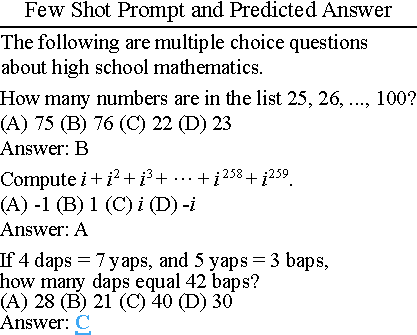
\includegraphics[width=\textwidth]{figures/few_shot_explainer_line.pdf}
\caption{An example of few-shot learning and inference using GPT-3. The \textcolor{rightblue}{blue} underlined bold text is the autocompleted response from GPT-3, while the preceding text is the user-inputted prompt. In this 2-shot learning example, there are two instruction examples and one initially incomplete example. On average, GPT-3 has low accuracy on high school mathematics questions.}\label{fig:fewshot}
\end{subfigure}\hfill%
\begin{subfigure}{.49\textwidth}
\centering
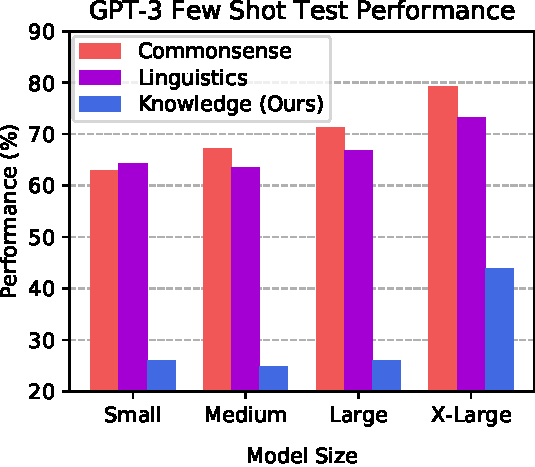
\includegraphics[width=\textwidth]{figures/test_juxaposition.pdf}
\caption{Performance on a commonsense benchmark (HellaSwag), a linguistic understanding benchmark (SuperGLUE), and the massive multitask test. On previous benchmarks, smaller models start well above random chance levels and exhibit more continuous improvements with model size increases, but on our test, GPT-3 moves beyond random chance with the largest model.}\label{fig:juxtaposition}
\end{subfigure}
\vspace{-13pt}
\end{figure}

% \begin{wrapfigure}{R}{0.5\textwidth}
% % 	\vspace{-30pt}
% 	\begin{center}
% 	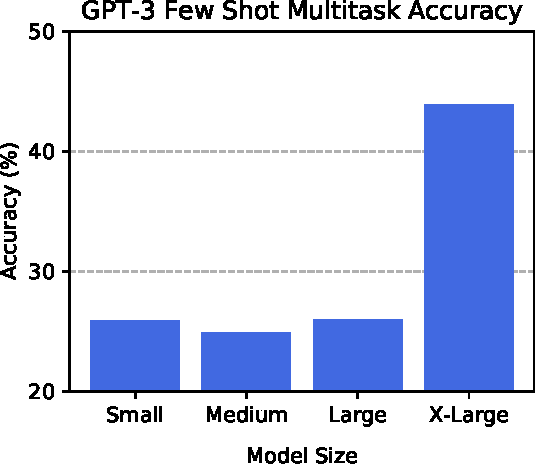
\includegraphics[width=0.5\textwidth]{figures/scale_and_accuracy.pdf}
% 	\end{center}
% 	\caption{Sizes and Accuracy. Random chance is 25\%.
%     }\label{fig:gptsizes}
% % 	\vspace{-10pt}
% \end{wrapfigure}

% Lorem Ipsum is simply dummy text of the printing and typesetting industry. Lorem Ipsum has been the industry's standard dummy text ever since the 1500s, when an unknown printer took a galley of type and scrambled it to make a type specimen book. It has survived not only five centuries, but also the leap into electronic typesetting, remaining essentially unchanged. It was popularised in the 1960s with the release of Letraset sheets containing Lorem Ipsum passages, and more recently with desktop publishing software like Aldus PageMaker including versions of Lorem Ipsum.



% \begin{figure}[t]
%     \centering
%     \vspace{-10pt}
%     \includegraphics[width=\textwidth]{figures/splash.pdf}
%     \caption{Given different scenarios, models predict widespread moral sentiments. Predictions and confidences are from a BERT-base model. The top three predictions are incorrect while the bottom three are correct. The final scenario refers to \citet{Bostrom2014SuperintelligencePD}'s paperclip maximizer. High performance on this task may enable the filtration of chatbot outputs that are needlessly inflammatory.
%     \looseness=-1}
%     \label{fig:splash}
%     \vspace{-10pt}
% \end{figure}
